%!TEX root = ../masters_thesis.tex

\section{Implementation} % (fold)
\label{sec:implementation}

HistoGlobe is a web-based Historical Geographic Information System. The data model and the conceptual interface model were introduced in the first sections of this chapter. This section introduces the underlying database model, a specific implementation of the data model, and the computational model that translates between the conceptual model and the database model. The first part provides an overview about the architecture of the system in section \ref{sub:system_architecture}. The remaining part of the section presents the implementation of the server-side and the client-side application in HistoGlobe.

% ------------------------------------------------------------------------------
\subsection{System Architecture} % (fold)
\label{sub:system_architecture}

HistoGlobe uses a classic client-server architecture of a web-based information system. The user opens the application in a Web browser, the \emph{client} side of the system, and interacts with it through the user interface. The web \emph{server} is a remote computer that hosts the database and the middleware. The user interacts with the interface and the client-side application sends a request for new data to the web server. The middleware checks the request and sends it as a query to the database to obtain the required data. It then transforms the data and sends it back to the client. The interface shows the new information.

\begin{figure}[H]
  \vspace{1em}
  \centering
  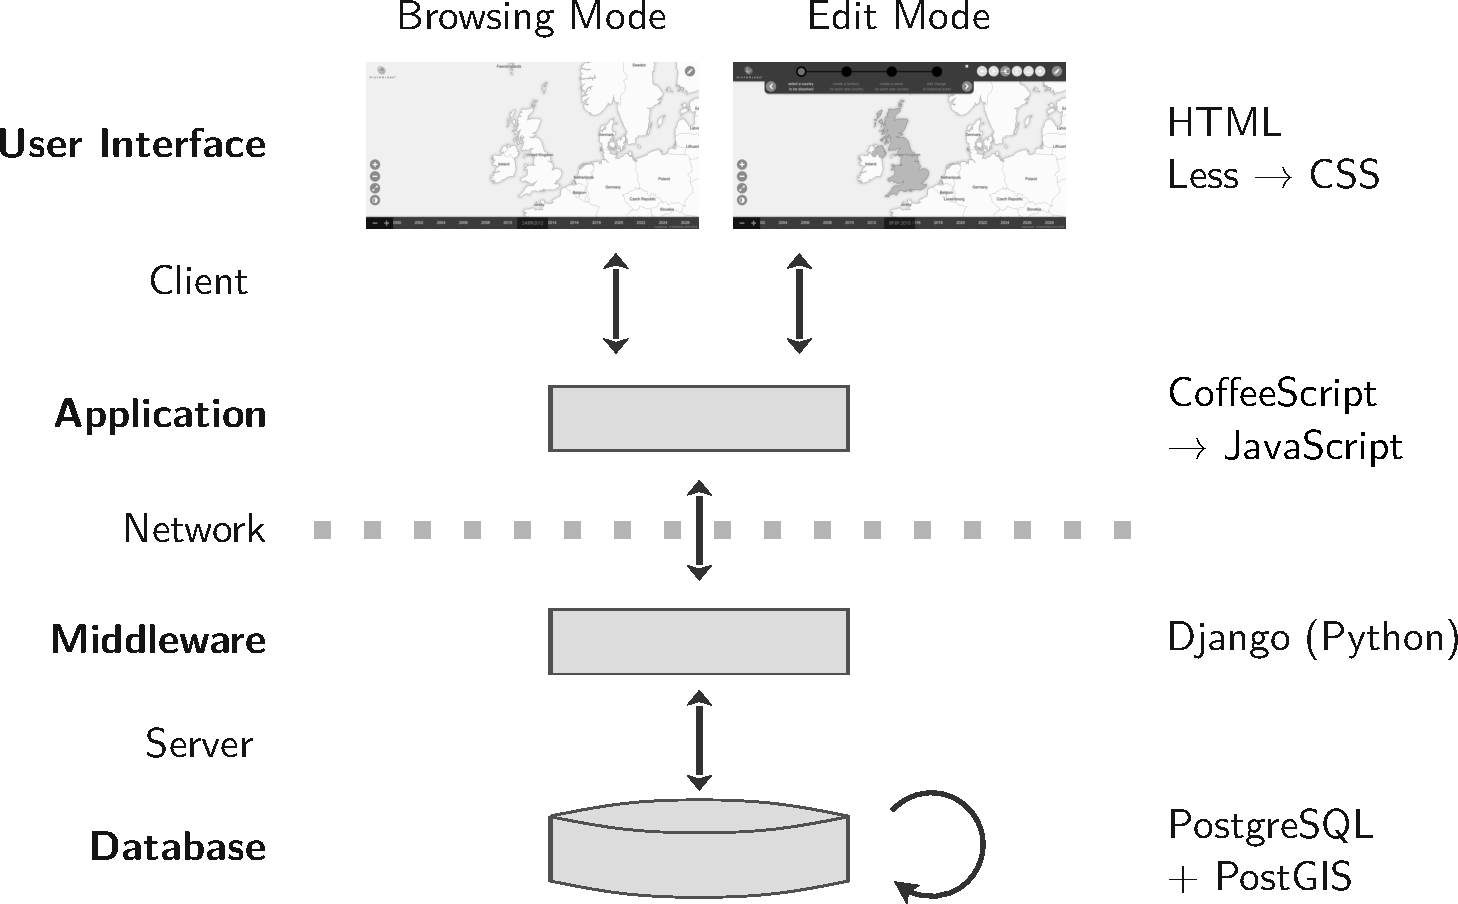
\includegraphics[width=0.66\textwidth]{graphics/development/implementation/system_architecture}
  \caption{The system architecture of HistoGlobe}
  \label{fig:system_architecture}
\end{figure}

This clear separation between data, application and user interaction in the system follows directly from the \emph{model-view-controller} pattern. One part can be changed independently from the others. If the 2D map is replaced by a 3D globe, only the view changes, but the middleware and the database can stay untouched. Likewise, the implementation of a new database technology has no consequences to the view.

% subsection system_architecture (end)

% ------------------------------------------------------------------------------
\subsection{Server-Side Application} % (fold)
\label{sub:server_side_application}

The underlying Hivent model is implemented on the server-side of the application. HistoGlobe uses \emph{Django}
\footnote{
  \emph{Django},
  The Web framework for perfectionists with deadlines,
  URL: \url{https://www.djangoproject.com/},
  accessed on: 27.05.2016
},
a free and open-source web framework combined with \emph{PostgreSQL}
\footnote{
  \emph{PostgreSQL:},
  The world's most advanced open source database,
  URL: \url{http://www.postgresql.org/},
  accessed on: 31.10.2015
},
which was introduced in section \ref{par:object_relational_dbms}. This allows HistoGlobe to take advantage of object-oriented concepts in a stable and fast relational database. Since the database is using a lot of geospatial data, \emph{PostGIS}
\footnote{
  \emph{PostGIS},
  Spatial and Geographic Objects for PostgreSQL,
  URL: \url{http://postgis.net/},
  accessed on: 27.05.2016
}
is used as a spatial database extension for PostgreSQL. With these tools, the Hivent model from section \ref{sec:hivent_model}  was implemented in a database model shown in figure \ref{fig:database_model_er}. This is the final result of a highly iterative process that was subject to several improvements and adaptations to new requirements introduced in the human-centered design process. The model is structured in two parts: the lower part of the Areas and the upper part of the Hivents and the historical changes.

\begin{figure}[ht]
  \centering
  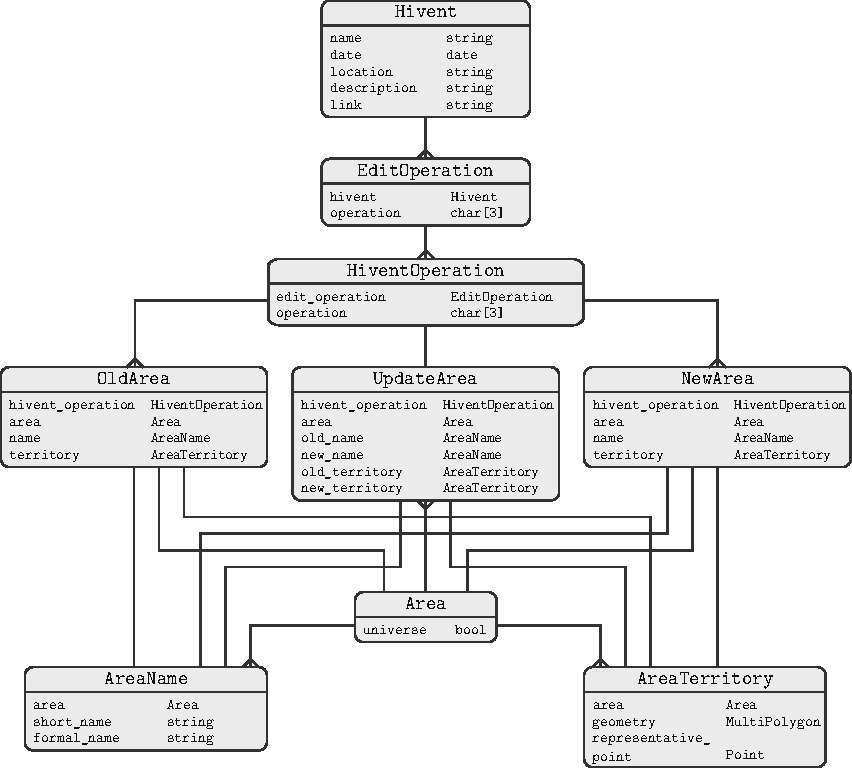
\includegraphics[width=0.9\textwidth]{graphics/development/implementation/database_model}
  \caption{The Hivent Database Model}
  \small{Each entity additionally has an \texttt{id} attribute, which is omitted for simplification purposes.} \\
  \small{Simple arrows denote a \texttt{1:1}-relationship, branching arrows a \texttt{1:n}}
  \label{fig:database_model_er}
\end{figure}

% - - - - - - - - - - - - - - - - - - - - - - - - - - - - - - - - - - - - - - -
\paragraph{Semantic, Spatial and Thematic Domain} % (fold)
\label{par:semantic_spatial_and_thematic_domain}

The Hivent model introduces Areas as visible entities on the map with a name and a territory. In the database model they are represented by:

\begin{enumerate}
  \item \texttt{Area}: Semantic domain defining one identical Area with potentially changing name and territory. The \texttt{universe} attribute is true for $\Omega$, for the other Areas it is false.
  \item \texttt{AreaTerritory}: Spatial domain. A polypolygon describes the \texttt{geometry} of the territory and a \texttt{representative\_point} the position of the name label on the map.
  \item \texttt{AreaName}: Thematic domain. It is defined by a \texttt{short\_name} and a \texttt{formal\_name}.
\end{enumerate}

% paragraph semantic_spatial_and_thematic_domain (end)

% - - - - - - - - - - - - - - - - - - - - - - - - - - - - - - - - - - - - - - -
\paragraph{Temporal Domain} % (fold)
\label{par:temporal_domain}

The main idea of the model is that the Areas can change over time. These changes are introduced by \texttt{Hivents}, the main entity of the eponymic model with five attributes: the \texttt{name} and a textual \texttt{description} of the Hivent, the point in time when the Hivent happened (\texttt{date}), the Hivent \texttt{location} as a simple string and a \texttt{link} (URL) to the related article, serving as a historical source.
Each Hivent consists of a set of \texttt{EditOperation}s introduced by the user.
They are an abstraction layer in the Hivent model between the \texttt{Hivent} and the \texttt{HiventOperation}s.
The operations replace a set of \texttt{OldArea}s with a set of \texttt{NewArea}s and might update the name or the territory of one specific \texttt{UpdateArea}.

% paragraph temporal_domain (end)


\begin{figure}[ht]
  \vspace{1.5em}
  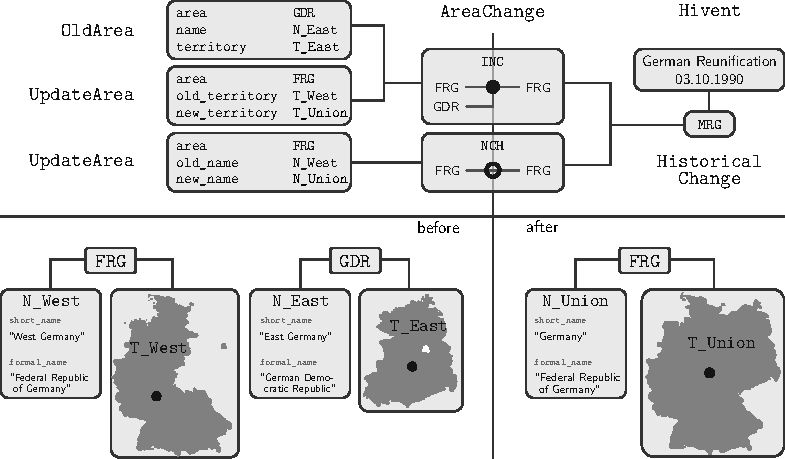
\includegraphics[width=0.9\textwidth]{graphics/development/implementation/example_reunification}
  \caption{Visualization of the German Reunification in the Hivent Database Model}
  \label{fig:database_example_reunification}
\end{figure}

Figure \ref{fig:database_example_reunification} shows the Hivent database model using the example of the German Reunification on 03.10.1990. Before 1990, there were the Areas \texttt{GDR} (``German Democratic Republic'', East Germany) and \texttt{FRG} (``Federal Republic of Germany'', West Germany). A user introduced a (\texttt{MRG}) operation in the Edit Mode between \texttt{FRG} and \texttt{GDR}. The new Area received the short name ``Germany'' and the same formal name ``Federal Republic of Germany'', previously held by West Germany. Internally, the Edit Mode translates this to an \texttt{INC} of \texttt{GDR} into \texttt{FRG} and a subsequent \texttt{NCH} of \texttt{FRG}. One Area ceases, one Area is updated twice and no new Area is created.

% - - - - - - - - - - - - - - - - - - - - - - - - - - - - - - - - - - - - - - -
\paragraph{Initial Dataset} % (fold)
\label{par:initial_dataset}

Section \ref{sub:data_sources} explained the lack of data about historical countries. It is beyond the scope of this thesis to create a large testing dataset with the historical countries in the world. The initial dataset consists of the following countries, their names and borders: the 193 UN members and 2 observer states -- created by \texttt{CRE} operation -- and seven countries with limited international recognition: Kosovo, Transnistria, South Ossetia, Abkhazia, Nagorno-Karabakh, Somaliland and Sahrawi Arab Democratic Republic. The issue regarding international recognition is explained in section \ref{par:un_non_members_with_limited_recognition}. Seven Areas were created by a \texttt{SPL} operations from their homeland on the day of their declaration of independence.

% paragraph initial_dataset (end)

% - - - - - - - - - - - - - - - - - - - - - - - - - - - - - - - - - - - - - - -
\paragraph{Middleware} % (fold)
\label{par:middleware}

The Django web framework provides \emph{view} classes that receive requests from the client, processes them, queries the necessary data from the database and returns an \texttt{HttpResponse} back to the client. In the naive implementation of the system, the middleware provides only two views for the following two use cases:

\begin{enumerate}
  \item \textbf{\texttt{get\_all}} is called by the client upon initializing the web service. The server responds to this \texttt{HttpRequest} with all data from the database in a single \emph{JSON} object.
  \item \textbf{\texttt{save\_edit\_operation}} is called by the client after an edit operation has been completely created in the Edit Mode. In the last step, the client assembles the relevant data: the associated \texttt{Hivent} and \texttt{HiventOperation}s, data about each \texttt{OldArea}, \texttt{UpdateArea} and \texttt{NewArea}. The view checks the data for integrity and stores it in the database. The method returns a confirmation to the client and a set of final \texttt{id}s for the entities stored in the database.
\end{enumerate}

% paragraph middleware (end)

% subsection server_side_application (end)

% ------------------------------------------------------------------------------
\subsection{Client-Side Application} % (fold)
\label{sub:client_side_application}

The main application of HistoGlobe runs on the client. As introduced in section \ref{sec:histoglobe}, the software is built upon a modular system. The modules used in this this implementation of HistoGlobe are emphasized in \textbf{bold} in the class diagram in figure \ref{fig:class_diagram}. The remaining classes were instantiated at run time by one of the seven modules. The classes are structured by their functionality regarding the Model-View-Controller pattern.

\begin{sidewaysfigure}[p]
  \centering
  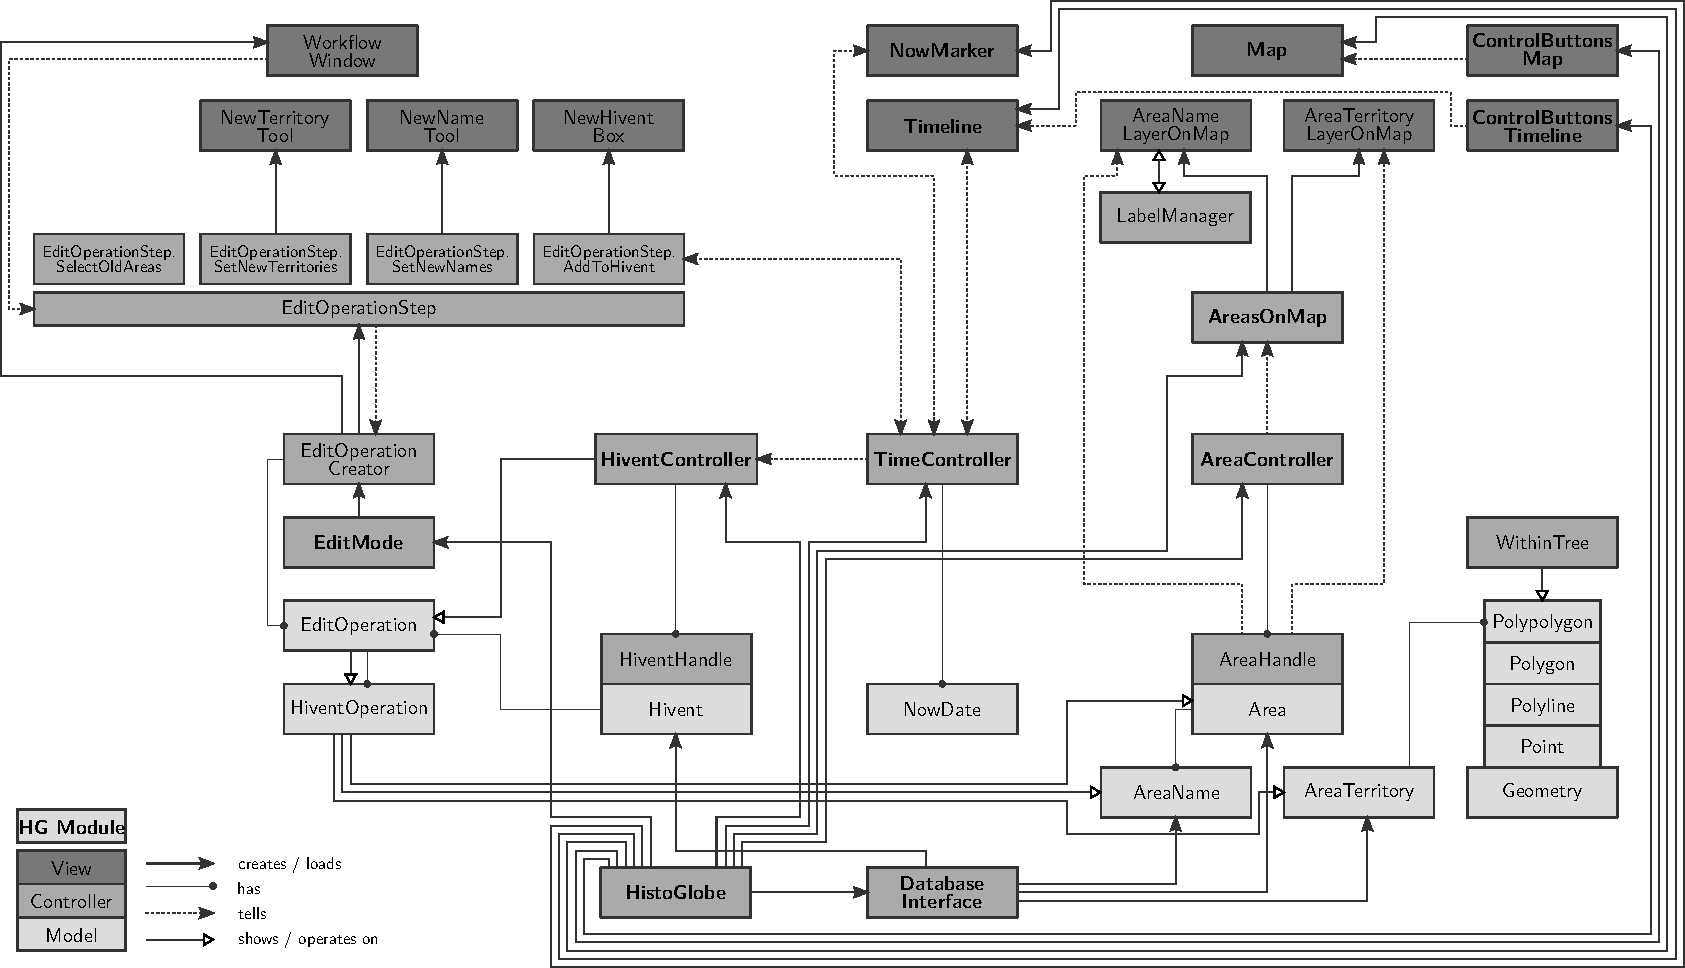
\includegraphics[width=0.95\textwidth]{graphics/development/implementation/class_diagram}
  \vspace{1em}
  \caption{Modules and classes in HistoGlobe}
  \label{fig:class_diagram}
\end{sidewaysfigure}

\newpage % forces the figure to be on the next page, because [H] does not work
% - - - - - - - - - - - - - - - - - - - - - - - - - - - - - - - - - - - - - - -
\paragraph{Initialization} % (fold)
\label{par:initialization}

The main HistoGlobe instance at the bottom initializes all modules, mainly the interface elements, the controllers and the \texttt{DatabaseInterface}. This class communicates with the middleware as seen in section \ref{par:middleware}. It loads data from the database and stores data in it. Initially, each \texttt{Hivent} and the related \texttt{EditOperation}s are created. Each \texttt{HiventOperation} is assembled by its associated set of \texttt{OldArea}s, \texttt{NewArea}s and the \texttt{UpdateArea} from the database model in  figure \ref{fig:database_model_er}. Afterwards, each \texttt{Area}, \texttt{AreaName} and \texttt{AreaTerritory} is loaded. A double-link is established to their associated \texttt{HiventOperation}s via the \texttt{startOperation}, \texttt{updateOperation} and \texttt{endOperation}.

% paragraph initialization (end)

% - - - - - - - - - - - - - - - - - - - - - - - - - - - - - - - - - - - - - - -
\paragraph{Execution of historical changes} % (fold)
\label{par:executing_historical_changes}

HistoGlobe visualizes time on the interactive \texttt{Timeline} and the \texttt{NowMarker} showing the current date of the application: The \texttt{NowDate}. Both view classes can manipulate the current date by moving the \texttt{Timeline} or entering a date. The \texttt{TimeController} stores the \texttt{NowDate} and tells all other modules if the current visualization has changed.

\begin{figure}[ht]
  \vspace{1em}
  \centering
  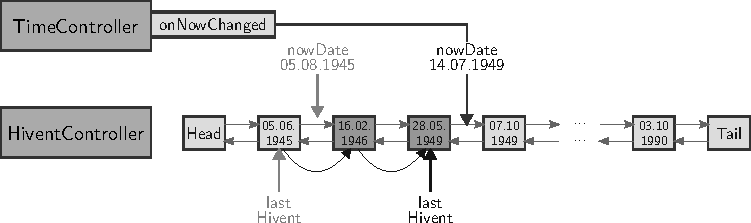
\includegraphics[width=0.9\textwidth]{graphics/development/implementation/hivent_controller}
  \caption{Detecting the next Hivent that happens in the HiventController}
  \label{fig:hivent_controller}
\end{figure}

The core of the Hivent-based implementation is the \texttt{HiventController}. Figure \ref{fig:hivent_controller} illustrates how it works: The controller stores a reference to each \texttt{Hivent} chronologically in a doubly-linked list, i.e.\ each \texttt{Hivent} knows the historically next and previous \texttt{Hivent}. Additionally, the controller stores a pointer to the last \texttt{Hivent} that has happened and a copy of the current date in the list. It listens to the \texttt{TimeController} -- if the \texttt{NowDate} changes, the \texttt{HiventController} checks if the next \texttt{Hivent} has happened. It compares this new date with its current date and checks if \texttt{Hivent.date} is in between these two dates. If this is the case, the \texttt{Hivent} happens and each \texttt{EditOperations} associated to this \texttt{Hivent} is executed on the map. The \texttt{HiventController} updates the pointer to the \texttt{Hivent} and checks for the next one until the next \texttt{Hivent} is outside this time span. If the \texttt{nowDate} from the \texttt{TimeController} is before the current date of the \texttt{HiventController}, it checks the \texttt{Hivents} backwards through the list and executes all the \texttt{EditOperations} backwards. This simple data structure effectively and efficiently manages temporal changes of \texttt{Area}s on the map.

The initialization of the system works as follows: all \texttt{Hivent}s in the list from the beginning until the \texttt{NowDate} of the \texttt{TimeController} are happening one after the other.

An \texttt{EditOperation} executes all its related \texttt{HiventOperations}. The main part of its source code, the \texttt{execution} function, is shown in listing \ref{lst:hivent_operation}. If an \texttt{HiventOperation} is to be executed forwards, then it happens in the following three steps:

\begin{enumerate}
  \item For each \texttt{newArea}, the \texttt{AreaName} and the \texttt{AreaTerritory} that the \texttt{Area} has in the moment are historically created and associated to the \texttt{Area}. Afterwards, the \texttt{Area} is shown on the map. The \texttt{AreaHandle} associated to the \texttt{Area} has a function that shows the associated \texttt{AreaNameLayerOnMap} and \texttt{AreaTerritoryLayerOnMap}.
  \item For each \texttt{oldArea}, the opposite happens: the name and territory are detached from the \texttt{Area} and the \texttt{AreaHandle} hides the \texttt{Area} from the map.
  \item In the \texttt{updateArea} the \texttt{AreaName} or \texttt{AreaTerritory} is replaced with the \texttt{newName} or \texttt{newTerritory}, respectively. The \texttt{update} method of the \texttt{AreaHandle} updates the respective layers on the map.
\end{enumerate}

If the operation happens backwards, \texttt{oldAreas} and \texttt{newAreas} are swapped and the \texttt{updateArea} instead uses the \texttt{oldName} or \texttt{oldTerritory}, respectively. This is the same for all five operations.

\begin{center}
\begin{minipage}[t]{0.9\textwidth}
\begin{lstlisting}[language=coffeescript,
  caption=Execution of an \texttt{HiventOperation} in forward direction,
  label=lst:hivent_operation]
class HiventOperation
    #... initialization of the member variables

    @oldAreas   = []  # {area, name, territory}
    @newAreas   = []  # {area, name, territory}
    @updateArea = {}  # {area, oldName, newName, oldTerritory, newTerritory}

  execute: (direction) ->

    if direction is 1

      for newArea in @newAreas
        newArea.area.name =       newArea.name
        newArea.area.territory =  newArea.territory
        newArea.area.handle.show()

      for oldArea in @oldAreas
        oldArea.area.name =       null
        oldArea.area.territory =  null
        oldArea.handle.hide()

      if @updateArea
        if @updateArea.newName
          @updateArea.area.name =      @updateArea.newName
        if @updateArea.newTerritory
          @updateArea.area.territory = @updateArea.newTerritory
        @updateArea.area.handle.update()
\end{lstlisting}
\end{minipage}
\end{center}

% paragraph executing_historical_changes (end)

% - - - - - - - - - - - - - - - - - - - - - - - - - - - - - - - - - - - - - - -
\paragraph{EditMode} % (fold)
\label{par:editmode}

The Edit Mode is the main contribution of this thesis to the HistoGlobe project.
Its interface was previously introduced in section \ref{sub:web_based_prototype} and its implementation is briefly explained here. When the user clicks an edit operation button in the edit mode interface, internally a \texttt{EditOperationCreator} sets up the \texttt{WorkflowWindow} in the interface and the first \texttt{EditOperationStep} for this operation. Each of the four steps have different tasks that were explained in section \ref{sub:edit_workflow}. Throughout the workflow, the \texttt{EditOperationCreator} stores the data for the operation (selected old Areas, newly created Areas, update Areas, including the old and new territories and names) in an object. Each step can access this object and manipulate its content.

\begin{enumerate}

  \item \texttt{SelectOldAreas}: The map is set in a \texttt{selectionMode} that requires the user to select a certain number of old Areas for the edit operation, i.e.\ one Area for \texttt{SPL}, \texttt{REN} and \texttt{CES}, one or two Areas for \texttt{CHB} and infinitely many Areas for \texttt{MRG}.

  \item \texttt{CreateNewTerritories}: The map is set into an \texttt{editMode} that prevents any selection of existing Areas except for the ones that are manipulated. For each Area that is created or updated in this operation, the user needs to create the new \texttt{AreaTerritory} of the Area in form of a polypolygon with the \texttt{NewTerritoryTool}:
  \begin{itemize}
    \item[\texttt{CRE}]
      Create one territory $B^T$, that is the territory of the new \texttt{Area} $B$.
      Check with the territory $A^T$ of each existing Area $A$ if the territories intersect ($A^T \cap B^T \neq \emptyset$).
      If they do, the territory $A^T$ is updated by subtracting the new territory $B^T$ from it via the complement (difference): $A^T = A^T \setminus B^T$.
      If the resulting territory $A^T = \emptyset$ it means that $A$ is completely covered by $B$, so it is entirely incorporated into $B$ and set as an old Area of the operation.
      If not, the territory of $A$ is updated with $A^T$ and $A$ is
      set as an updated Area of this step that cedes parts of its territory to $B$.
    \item[\texttt{MRG}]
      This step happens automatically without any user interaction. The new territory $B^T$ is created by the cascaded union of the territories $A^T_i$ of the selected Areas $A_i \in A$ from the first step: $B^T = \bigcup\limits_{i=1}^n A^T_i$. It is set as the territory of $B$.
    \item[\texttt{SPL}]
      Each desired new Area $B_i \in B$ needs a territory $B_i^T$. This is obtained by intersecting the temporary territory $T_i$ that the user has created in the \texttt{NewTerritoryTool} with the territory of the selected Area: $B_i^T = A^T \cap T_i$. This is repeated until the entire territory $A^T$ is completely distributed among $B_i \in B$.
    \item[\texttt{CHB}]
      If the user selected only one old Area $A_1$ in the first step, then territory $T_1$, created by the \texttt{NewTerritoryTool} in this step, will be set as the new territory of $A_1$. The surrounding Areas are handled in the same way as in the \texttt{CRE} operation. If two neighboring Areas $A_1$ and $A_2$ were selected, the new territories are obtained like this: $T_1$ is seen as the basis of territory $A_1^T$. It is temporarily unified with its neighbor $A^T_2$ to $B^T = A_1^T \cup A_2^T$. Then the new territory $A_1^T$ is cut out from this temporary union with an intersection: $A_1^T = B^T \cap T_1$. $A_2$ receives the remaining part as its new territory: $A_2^T = B^T \setminus T_1$.
  \end{itemize}
  No new territories are created in \texttt{REN} and \texttt{CES}.

  \item \texttt{CreateNewNames}: For each Area that is created or updated in this operation, the user needs to create a new \texttt{AreaName} with a short name and formal name using the draggable \texttt{NewNameTool}. The user writes the new names or selects them from the suggestions. Not only the name will be taken from the \texttt{NewNameTool}, but also the center position of the box will be the new \texttt{representative\_point} of the \texttt{AreaTerritory}. The user decides where the name of the Area should be positioned. This avoids the information visualization problem of automatic label placement.

  \item \texttt{AddToHivent}: The user creates a new Hivent using the \texttt{NewHiventBox} or selects an existing Hivent to which the edit operation is added to.

\end{enumerate}

It was especially difficult to design each action to be fully reversible. For that purpose, an associated inverse of the action was stored in an \texttt{UndoManager} that works like a stack. If the user clicks the back button in the Workflow Window, the last action of the stack gets executed. When the last stage of the workflow (\texttt{AddToHivent}) is completed, the \texttt{EditOperationCreator} assembles the \texttt{HiventOperations} from the data gathered in the task. It sends it to the server along with the associated \texttt{Hivent} and finishes the operation.


% paragraph editmode (end)

% - - - - - - - - - - - - - - - - - - - - - - - - - - - - - - - - - - - - - - -
\paragraph{WithinTree} % (fold)
\label{par:within_tree}

The \texttt{NewTerritoryTool} in the second step of the workflow has to ensure that the drawn polygons are not self-intersecting and that no two polygons for one territory partially overlap each other. If they fully overlap, then they create holes in the polygon. A polygon consists of one \emph{outer ring}, a closed polyline forming the boundary of the polygon, and a set of \emph{inner rings}, closed polylines defining the holes in the polygon and representing first-order enclaves. Second-order enclaves are new polygons that happen to be positioned inside the inner rings of the other polygon. They can themselves have inner rings, which represent third-order enclaves, etc. In order to support nested holes, the \emph{WithinTree} is introduced. The idea is to set up a hierarchical structure of polygons that contain each other. An example WithinTree for a random set of polygons can be seen in figure \ref{fig:within_tree}.

\begin{figure}[ht]
  \vspace{1em}
  \centering
  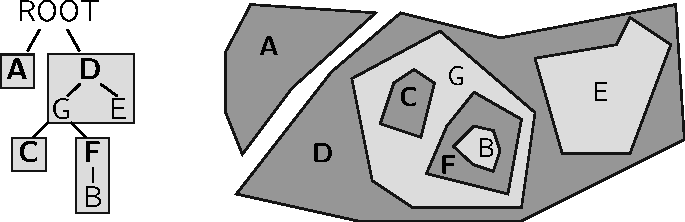
\includegraphics[width=0.6\textwidth]{graphics/development/implementation/within_tree}
  \caption{The WithinTree (left) for the set of polygons (right)}
  \label{fig:within_tree}
\end{figure}

The algorithm for inserting a polygon as a node into the tree is shown in listing \ref{lst:within_tree_insertion}. After the tree has been set up, the correct structure of polygons can be obtained by traversing the tree in the following custom order:

\begin{compactenum}
  \item Remove the first child $F$ of the root node and all its children $C$ from the tree.
  \item Insert each child of each $C$ as a direct child of the root node.
  \item Create a new polygon with $F$ as the outer ring and each $C$ as an inner ring.
  \item Repeat until the tree is empty.
\end{compactenum}



\begin{center}
\begin{minipage}[t]{0.9\textwidth}
\begin{lstlisting}[language=coffeescript,
  caption=Insertion of a polygon node into the WithinTree,
  label=lst:within_tree_insertion]
insert: (newNode, parentNode) ->

  ## PREPARATION
  # case 1) newNode also in 1 child of parentNode  -> withinChild
  # case 2) 1+ children of parentNode in newNode   -> containChildren
  # case 3) no hierarchical relation between newNode and any other node

  withinChild =     null
  containChildren = []

  for childNode in parentNode.children

    if newNode.isWithin(childNode)                  # check if case 1)
      withinChild = childNode
      break # no other hierarchical relation to any other child possible

    else if childNode.isWithin(newNode)             # check if case 2)
      containChildren.push(childNode)

  ## EXECUTION

  if withinChild                                    # case 1)
    @insert(newNode, childNode)

  else                                              # cases 2 and 3)
    # newNode is not in any child of parentNode => place it underneath
    @_nodes.push(newNode)
    newNode.setParent(parentNode)
    parentNode.addChild(newNode)

    for containChild in containChildren             # case 2)
      # => detach from parent node and place them as children of newNode
      containChild.setParent(newNode)
      newNode.addChild(containChild)
      parentNode.removeChild(containChild)
\end{lstlisting}
\end{minipage}
\end{center}

% paragraph within_tree (end)

% - - - - - - - - - - - - - - - - - - - - - - - - - - - - - - - - - - - - - - -
\paragraph{LabelManager} % (fold)
\label{par:labelmanager}

A major visualization problem that was sufficiently solved in the thesis is the label collision problem. Each active Area has both a territory and a name that should be shown on the map. Axiom \ref{axm:unique_coverage} states that no territories can overlap, so they can all be shown. This is not true for the names of the Areas. The \texttt{short\_name} of the \texttt{AreaName} is placed as a label in the \texttt{representative\_point} of the \texttt{AreaTerritory}. Labels can overlap, because they can extend beyond their territory. To avoid this, some labels have to be hidden. A \texttt{LabelManager} decides for each label if it is shown or hidden. Each label gets an additional set of attributes:

\begin{compactitem}
  \item \texttt{isVisible}: Status variable if the label is shown or not
  \item \texttt{priority}: The importance of the label determined by the size of the territory
  \item \texttt{boundingBox}: Width and height of the text
  \item \texttt{coveredBy}: A list of higher-priority labels that cover this label
  \item \texttt{covers}: A list of lower-priority labels that are covered by this label
\end{compactitem}

Label $A$ covers label $B$ if their bounding boxes intersect and $A$ has a higher priority. The labels are stored in a doubly-linked \texttt{labelList} in descending priority order. The algorithm is based on the following heuristic: \emph{A label is shown unless it is covered by a higher-priority label}.

When a new label is introduced, it is inserted into the \texttt{LabelManager} in the following way:
Each label has to be inserted in the correct position in the \texttt{labelList}. Therefor, it is compared with each existing label in descending priority if it overlaps and if the priority is still higher.
As soon as the first label with a lower priority is found, the new label is inserted before this label in the list. If there was a higher-priority label before that covered it, the new label is hidden -- otherwise it is shown. In the latter case all lower-priority labels are checked if they are covered by the new label -- if they are, then they are hidden.

If an Area also ceases, its name is also hidden from the map. Additionally, the old label is removed from the \texttt{labelList}. Each label that was previously covered by the old label is not covered by it any more. If no other label still covers it, the label can be shown.

If the user zooms the map, the \texttt{LabelManager} has to update the visibility status of each label. Zooming in  means that each label has more space to its neighbors. No label has to be hidden, but hidden labels can be shown if they are not covered by any other label any more. Vice versa, if the user zooms out, the labels have less space to their neighbors. No label can be become visible, but a visible label needs to be hidden if it is covered by at least one other label.

\begin{figure}[ht]
  \vspace{1em}
  \centering
  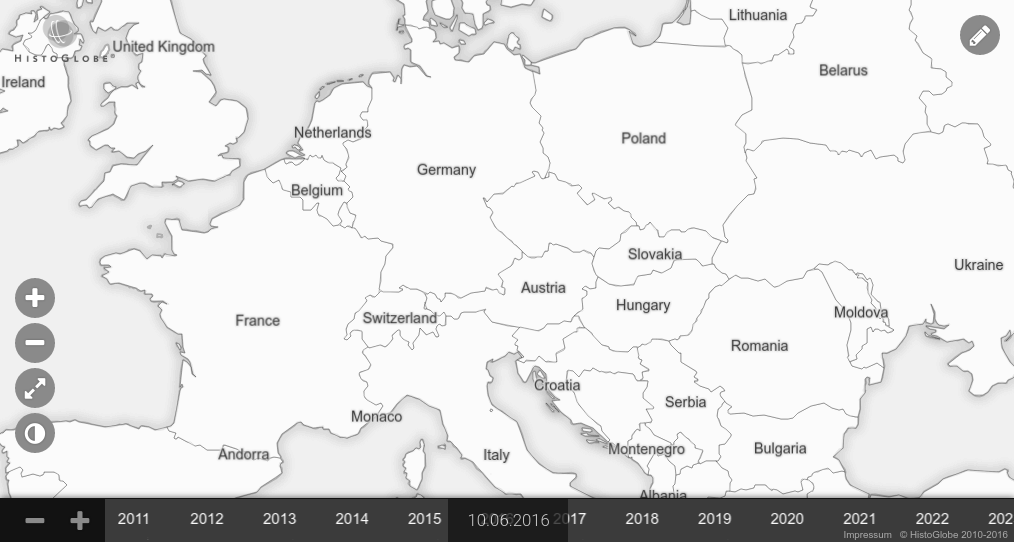
\includegraphics[width=0.9\textwidth]{graphics/development/implementation/label_manager.png}
  \caption{The resulting labels on the map in Europe 2016}
  \label{fig:label_manager}
\end{figure}

Figure \ref{fig:label_manager} shows the result of the \texttt{LabelManager} on the map of Europe in 2016. It is obvious that no two labels collide. This was the main motivation for the algorithm. Also, the labels of the large countries Ukraine, Poland, Germany, France and the United Kingdom are shown. However, the label ``Czech Republic'' is hidden, because its bounding box intersects with the label ``Germany''. On the other hand the labels of Monaco and Andorra are shown, although they are rather insignificant. But since there is enough space around them, they are shown.
If a short name has more than one word, automatic line breaks at could be inserted at reasonable positions, e.g.\ ``Czech$|$Republic''. With this possible extension, more labels could be shown.
However, this is subject to future work.
The \texttt{LabelManager} sufficiently serves the purpose of this thesis.

% paragraph labelmanager (end)

% subsection client_side_application (end)

% section application (end)